% fig_creator_stats.tex  -  Memory files by normalized role family.
%   Horizontal bar chart, sorted descending.  Dark bars: roles in the
%   specialized-role taxonomy (\cref{tab:roles}).  Light bars: labels
%   outside it (chat, untagged bootstrap files, and a residual other
%   group: presenter 3, review sessions 2, user 1).
%   Bar length encodes file count; scale S = 0.034 cm per file (so the
%   x-tick at 150 sits at 5.10 cm).  Total = 453 (sum of the bars below).
% Requires: \usepackage{tikz} (loaded in preamble).
\begin{figure}[htbp]
\centering
\resizebox{0.66\textwidth}{!}{%
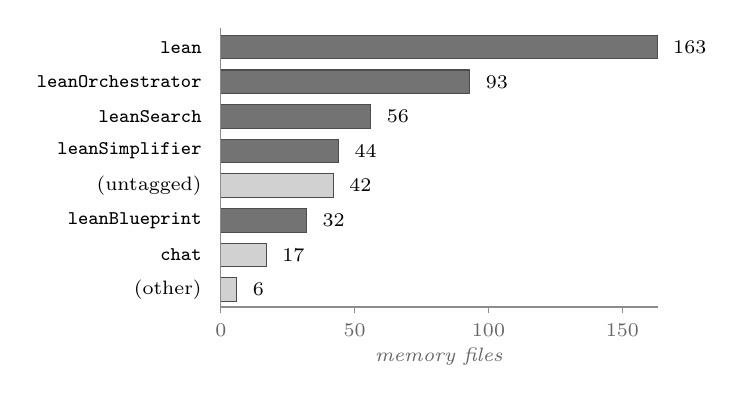
\begin{tikzpicture}[
    role/.style ={fill=black!55, draw=black!70, thin},
    other/.style={fill=black!18, draw=black!70, thin},
    cat/.style  ={font=\scriptsize, anchor=east},
    val/.style  ={font=\scriptsize, anchor=west},
    ax/.style   ={draw=black!45}
  ]

  %% ---- bars (y top to bottom, descending count) --------------------
  \filldraw[role]  (0,3.81) rectangle (5.542,4.11);
    \node[cat] at (-0.12,3.96) {\texttt{lean}};            \node[val] at (5.622,3.96) {163};
  \filldraw[role]  (0,3.37) rectangle (3.162,3.67);
    \node[cat] at (-0.12,3.52) {\texttt{leanOrchestrator}};\node[val] at (3.242,3.52) {93};
  \filldraw[role]  (0,2.93) rectangle (1.904,3.23);
    \node[cat] at (-0.12,3.08) {\texttt{leanSearch}};      \node[val] at (1.984,3.08) {56};
  \filldraw[role]  (0,2.49) rectangle (1.496,2.79);
    \node[cat] at (-0.12,2.64) {\texttt{leanSimplifier}};  \node[val] at (1.576,2.64) {44};
  \filldraw[other] (0,2.05) rectangle (1.428,2.35);
    \node[cat] at (-0.12,2.20) {(untagged)};               \node[val] at (1.508,2.20) {42};
  \filldraw[role]  (0,1.61) rectangle (1.088,1.91);
    \node[cat] at (-0.12,1.76) {\texttt{leanBlueprint}};   \node[val] at (1.168,1.76) {32};
  \filldraw[other] (0,1.17) rectangle (0.578,1.47);
    \node[cat] at (-0.12,1.32) {\texttt{chat}};            \node[val] at (0.658,1.32) {17};
  \filldraw[other] (0,0.73) rectangle (0.204,1.03);
    \node[cat] at (-0.12,0.88) {(other)};                  \node[val] at (0.284,0.88) {6};

  %% ---- axes --------------------------------------------------------
  \draw[ax] (0,0.66) -- (0,4.20);
  \draw[ax] (0,0.66) -- (5.55,0.66);
  \foreach \x/\t in {0/0, 1.70/50, 3.40/100, 5.10/150} {
    \draw[ax] (\x,0.66) -- (\x,0.58);
    \node[font=\scriptsize, text=black!60, anchor=north] at (\x,0.57) {\t};
  }
  \node[font=\scriptsize\itshape, text=black!60, anchor=north] at (2.77,0.26) {memory files};

\end{tikzpicture}%
}
\caption{Memory files by the agent role that last modified them (total $=453$). Dark bars are roles in the specialized-role taxonomy of \cref{tab:roles}; light bars are labels outside it: \texttt{chat}, untagged startup files from before the metadata was recorded, and a residual \texttt{other} group.}\label{fig:by_labels}
\end{figure}

